\section{Leitungen}
\subsection{Übertragungsleitung mit Last}
\makebox[0pt][l]{
    \begin{minipage}{\columnwidth}
        \centering
        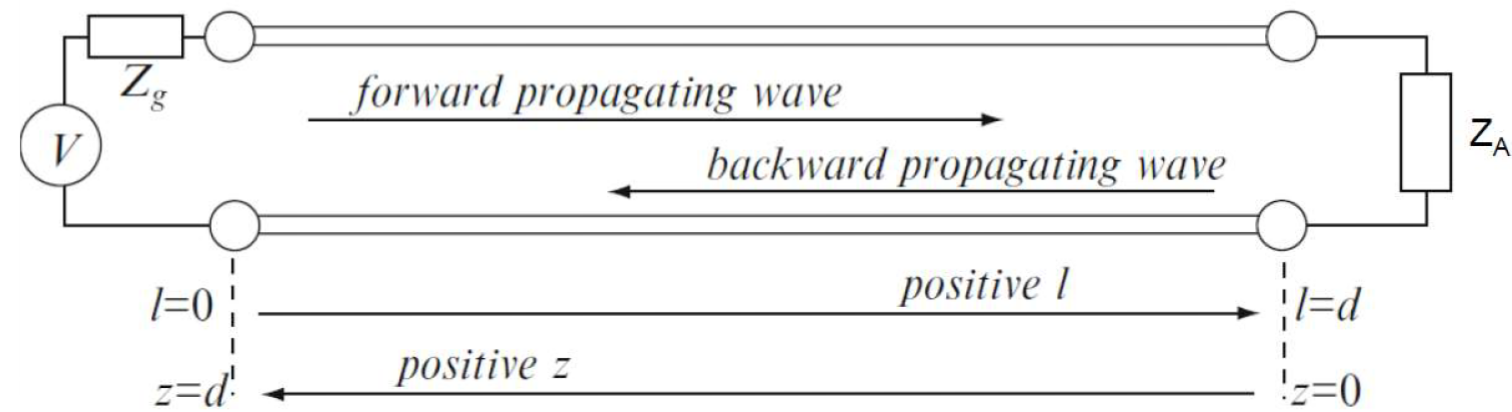
\includegraphics[width=1\columnwidth]{Figures/UebertragungleitungmitLast.png}
        \label{fig:Übertragungsleitung}
    \end{minipage}
}
\begin{align*}
     & U(z) = U^+ e^{\gamma z} + U^- e^{-\gamma z} = U^+ e^{\gamma d} + U^ - e^{-\gamma d}                        \\
     & I(z) = I^+ e^{\gamma z} + I^- e^{-\gamma z} = \dfrac{U^+}{Z_L}e^{\gamma d} - \dfrac{U^-}{Z_L}e^{-\gamma d} \\
     & \underline{z}_n = \dfrac{\underline{Z}_A}{Z_L}                                                             \\
     & \underline{r} = \dfrac{\underline{z}_n-1}{\underline{z}_n+1}= \dfrac{1-\underline{y}_n}{1+\underline{y}_n} \\
     & \underline{r}_A = \dfrac{\underline{Z}_A-Z_L}{\underline{Z}_A+Z_L}                                         \\
     & m = \dfrac{1-|\underline{r}|}{1+|\underline{r}|}
\end{align*}
\subsubsection{Refelxionsfaktor entlang einer Leitung}
\begin{align*}
    &r_E = r_A \cdot ^{-2\gamma l} = r_A \cdot e^{-2\alpha l}\cdot e^{-j2\beta l}\\
    &\alpha = -\dfrac{ln(r_A)}{2l} [Np/m]
    &\beta = \dfrac{\phi_2 -\phi_1}{2l} [rad/m]
\end{align*}

\subsubsection{Stehwellenverhältnis}
\begin{align*}
    SWR = \dfrac{U_{max}}{U_{min}} = \dfrac{I_{max}}{I_{min}} = \dfrac{1+|r(z)|}{1-|r(z)|}
\end{align*}
